\documentclass[main.tex]{subfile}

\begin{document}

\section{Nyquist Frequency} 
\label{sec:nyquist_frequency}

A given sinusoidal wave is represented mathematically as:

\begin{align}
  x(t) = A\sin{((\omega t + \phi))} + y
\end{align}
where $A$ is the amplitude, $\omega$ is the angular frequency, $\phi$ is the
phase shift, and $y$ is the y-axis offset. If an Analog-to-Digital-Converter (or
ADC) circuit is used to obtain a digital representation of the signal we then
have the cooresponding digital sinusoidal wave: 

\begin{align}
  x[n] = A\sin{(\omega \delta_{t} n + \phi)} + y \label{eq:sampledWave}
\end{align}
where $n$ is the n$^{th}$ sample and $\delta_{t}$ is the sampling time step size
which is obtained from the sampling frequency $f_s$ as $\delta_{t} =
\frac{1}{f_s}$. If the sampling frequency is lower than the frequency of the
wave being sampled then the aliasing affect occurs as follows.

First we observe that a sin wave is periodic every $2\pi$ and thus phase shifts
of $2\pi a$ have no change on the highway. Applying this principle to \eqref{sampledWave}
we obtain the following:

\begin{align}
  x[n] &= A\sin{(2\pi f \delta_{t} n + \phi)} + y \label{eq:sampledWave}
  \\&= A\sin{(2\pi f \delta_{t} n + 2\pi a + \phi)} + y
  \\&= A\sin{(2\pi \delta_{t} n (f + \frac{a}{n\delta_{t}})}) + y
\end{align}

Note that

% section nyquist_frequency (end)

\begin{figure}[H]
  \begin{center}
    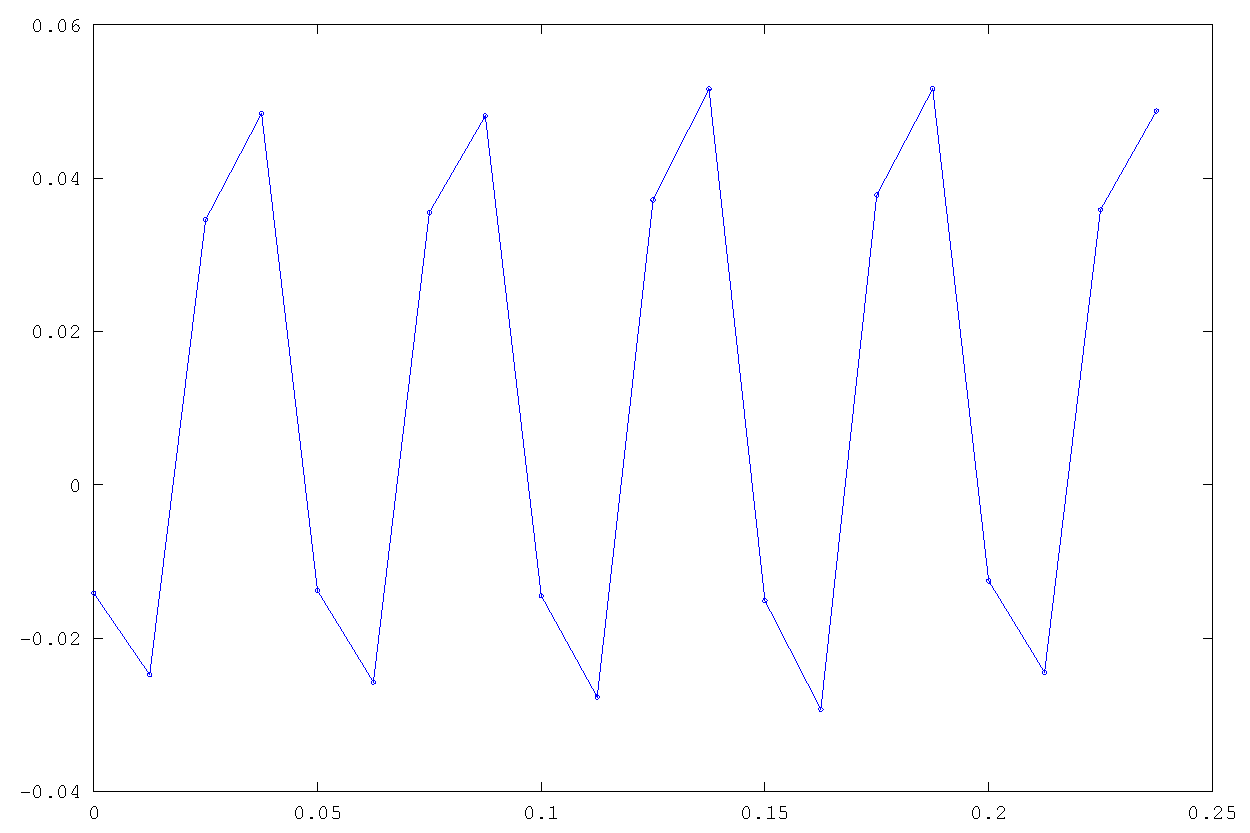
\includegraphics[width=\linewidth]{pt2_80Hz.pdf}
  \end{center}
  \caption{$80\dem{Hz}$ Measured Sine Wave}
  \label{fig:pt280hz}
\end{figure}

\begin{figure}[H]
  \begin{center}
    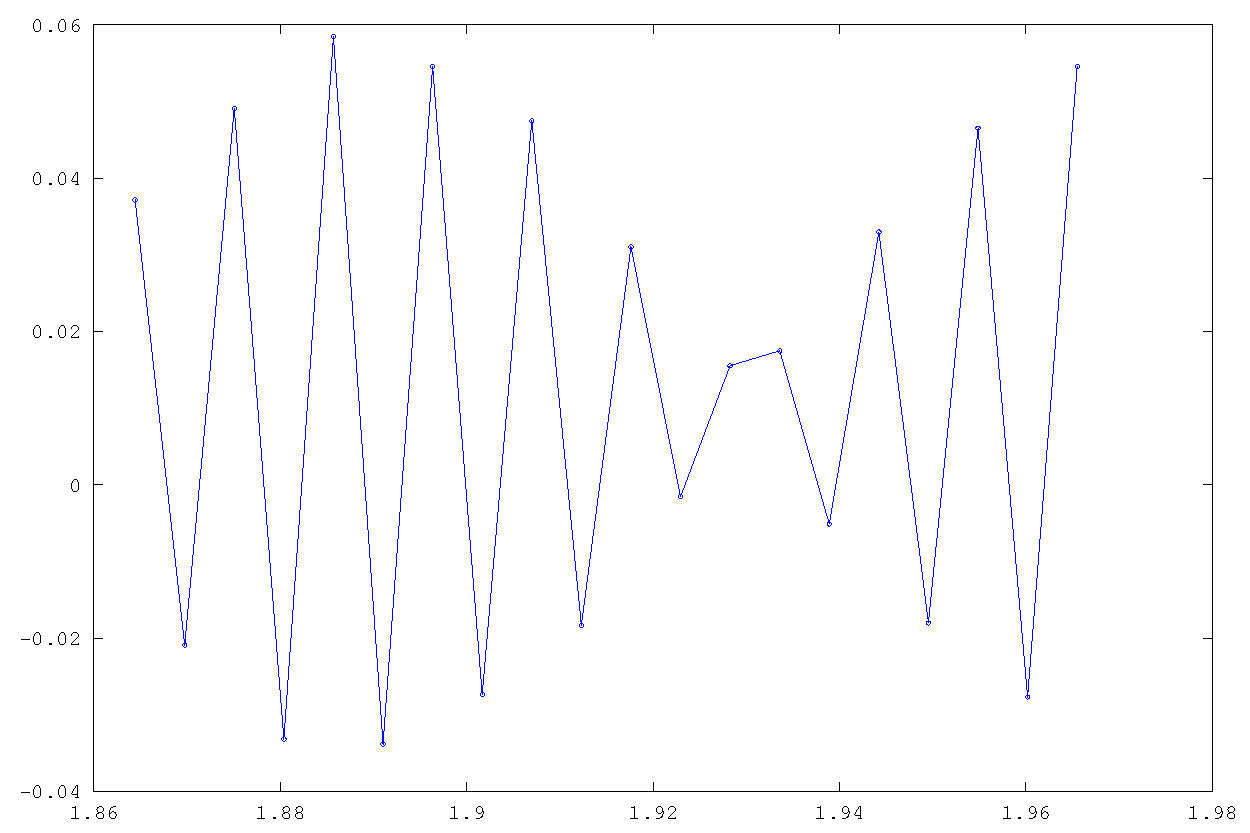
\includegraphics[width=\linewidth]{pt2_200Hz.pdf}
  \end{center}
  \caption{$200\dem{Hz}$ Measured Sine Wave}
  \label{fig:pt280hz}
\end{figure}
% document text goes here

\end{document}
